\section{Web scraping}
Web scraping is extracting structured data from websites. The term typically refers to automated processes implemented using a bot or web crawler. It is a form of copying, in which specific data is gathered and copied from the web, generally into a central local database or spreadsheet, for later retrieval or analysis \cite{webscrapingwiki}. \\
The first target that had to be accomplished to turn the Mercurio project and its analysis to an international version was the data collection of financial news from various sources using web scraping techniques. In particular, the websites that have been considered were: 
\begin{itemize}
\item \href{https://www.bloomberg.com}{bloomberg.com}
\item \href{https://www.nytimes.com}{nytimes.com}
\item \href{https://www.thisismoney.co.uk}{thisismoney.co.uk}
\item \href{http://money.cnn.com}{money.cnn.com}
\item \href{http://www.marketwatch.com}{marketwatch.com}
\item \href{http://www.reuters.com}{reuters.com}
%\item \href{http://www.investing.com}{investing.com}
\item \href{http://www.moneymorning.com}{moneymorning.com} 
\item \href{http://www.4-traders.com/}{4-traders.com}
\end{itemize}
An important distinction among the sources mentioned above is whether or not is required an ajax/javascript interaction with the user in the web page that arranges the articles under consideration. Those that do not involve these interaction will be treated in the "static websites" section, the leftovers in the "dynamic websites" section, with a focus on infinite scroll websites. \\ 
To manage this issue of the project, the Scrapy open source framework \cite{scrapyframework} has been used. 
\par
The creation of the project has been done with the command: "scrapy startproject tutorial" from command line interface; this will create the template composed with a series of folder for the implementation of spiders.
Once the project has been created, a single Spider \cite{scrapyspider} for each source has to be set up: they are the classes that define how a source will be scraped, and in particular, how to perform the crawling (i.e. follow links) and how to extract structured data from the page. The Spider's lifecycle varies a little between dynamic and static websites, but basically it starts by sending a request to URLs specified in starting\_url, afterwards it gets the data, stores it on some physical support (e.g. database, files) and finally crawls to another source or invokes some javascript commands and repeats. The single steps could be more or less complicated depending on the considered source. \\
In order to make the storing stage work, the Scrapy Item Pipeline \cite{scrapypipeline} has been used. It does a very simple task, once it receives an item that changes according to the source, it performs some action over it (i.e. store it).\\
Depending on the type of information that the website provides, the items that can be stored using the pipeline are two: "BriefItem", that contains a field for title, date, time, and an eventual URL where the news is better specified, and "NewsItem", which carries a value for title, authors, date, time, content and keywords. The former has been used when the use of the latter didn't make sense, due to a lack of information on the website, or due to the impossibility of retrieving it: for example, some websites (e.g. Marketwatch) provide a list of links to financial articles from many different websites, making out of the question to get the more specified data from such different website formats. The "date" saved for each news is synchronized on the UTC timezone by using the "pytz" library.

\begin{figure}[H]
\centering
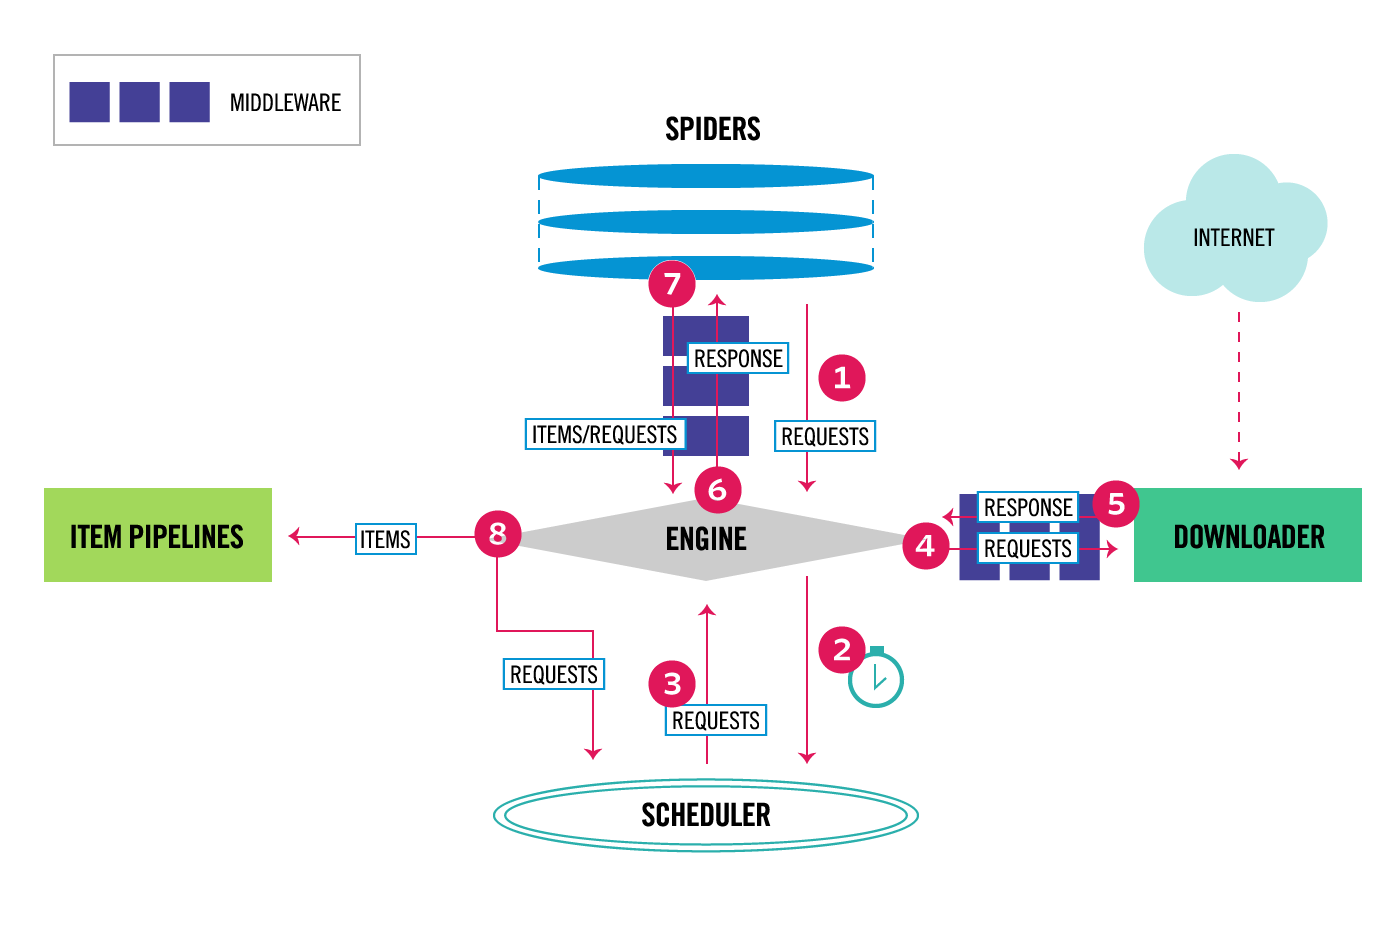
\includegraphics[width=\textwidth]{Architettura}
\caption{Architettura del framework di Scrapy}\label{fig:1}
\end{figure}

\subsection{Saving the data}
When it comes to saving the data there is a multitude of possibilities, ranging from a simple text file to a more structured database. 
At first, for testing purpose, the data has been saved in a tsv(i.e. tab separated values) textual file. Subsequently, in the deployment stage, it has been memorized on a database. For the management of the code it has been chosen to keep both the database and the files using a strategy pattern. This means that in order to test new scraping scripts in the future, it is possible to switch to the file methodology changing only few lines of code. 
\par
As it is shown on the architecture, the item(i.e. BriefItem or NewsItem) goes through a pipeline, but before that, it must be loaded with data.
The initialization of an item can be done with two methods:
\begin{itemize}
	\item Creating an item with its constructor;
	\item Using an item loader to fill the field of the item.\\
	This kind of object lets the developer define two preprocessing operations for each field of the item:
	\begin{itemize}
		\item input preprocessing, which provides a set of operations to be done when the data is filled inside the item loader (e.g. remove tags, remove escape characters, etc...)
		\item output preprocessing, which provides an operation to be done when the item is created (e.g. taking only the first data of that specific field if there are a lot of data or concatenating those strings gotten through scraping)
	\end{itemize}
\end{itemize}

\par While structuring and developing the scripts, no design pattern has been identified and used, except for the structure that the Scrapy framework itself already has. In fact the single steps that have to be performed have strong dependencies with  the websites' structure and the ways that they arrange the information. For instance, most of the scripts are really light in term of lines of code, and the majority of them regards mainly the way in which the websites arranges its information and articles (e.g. a set of <li> tags). The only model that came to mind is the Template method pattern \cite{templatepattern}, but it only introduces redundancy with the Scrapy framework structure. 
\subsection{Static sites}
Nytimes.com and marketwatch.com are the only sources considered that doesn't fall under this category: every other sites doesn't require any kind of interaction with the client. In particular, the remaining ones can be further split in the ones that needs to scraped by modifying a value in the URL (i.e. the page number of a certain section) and the ones for which their sitemap is used and analyzed to retrieve the links of the interested articles. 
\par
Investing.com and 4-traders.com are the sites that fall under the first of the two classes illustrated above. The parse method starts from a certain page number (zero) and retrieves the information require; after that, if necessary, another function that scrape the single articles is called (this happens in 4-traders.com). Finally, a request to the next page is done and the parse method will handle it.
% XML and sitemap scraper
\par 
\subsection{Dynamic sites}
This regards dynamic sites.
\subsubsection{Infinite scroll websites}
Scrolling was the type of interaction required with client in both sites mentioned above: an "infinite" page kept loading contents progressively while being scrolled. This led to various issues that have been faced and solved in different ways. \\
The only solution found on the internet with a brief research on different sites wasn't very smart w.r.t. used physical resources \cite{currentscrollsolution}: these simple scripts just run an infinite loop in which the driver executes some lines of javascript to scroll the page down. Although this could fit good for some application/sites that doesn't require nor make possible (due to the presence of shrunk content on the page) to execute many times the scroll, if many years of financial articles needs to be loaded it will lead to a waste of memory and a sensible slow down of the application, e.g.:  after a year of news scraped in \url{https://www.nytimes.com/section/business/dealbook}, the Spider decelerated to the point where the javascript code was executed every 5 minutes, while it takes near to 1 seconds in the beginning. This happens because all the page is kept in memory (with many images displayed) and the DOM gets bigger at every request(?). Always referring to the previous example, after 1 year of news scraped, Firefox was using around 1.5 Gigabytes of RAM. \\
The first way tried to bypass the problem, was using the browser in headless mode, that is without graphic interface, (to do this, an option of Selenium driver needs to be set up) but the issue persisted. \\
The second, and working, solution is to dynamically remove HTML code from the page while it's being scraped. This has been done in different ways that are going to be compared later in the paper. 
\par 
The first example of site, that we found, with the implementation the infinite scrolling is \url{https://www.nytimes.com/section/business/dealbook}. The solution adopted for scraping nytimes is based on open the site in smartphone mode for bypassing the infinite scrolling with the button "Show more". Indeed if you open the site in desktop mode the button "Show more" disappear after the first click, while in smartphone mode this effect doesn't exist. One time that the scraper setted the correct mode for opening the site, it removed the unnecessary static html code from the page and a while true loop started. The loop at first clicked on button, it took the new articles which is updated by the page and it yielded them to the pipeline for being save. After that the script removes all <li> tags are executed, in order to reduce the physical resources used by the page, and the loop is restarted. Although all this precautions the page after had updated at least two years it became slow and the time for scraping articles is increased, for this the perfect solution for using this scraper is putted it on server.   
\par 
Let's analyze the solution adopted for \url{https://www.marketwatch.com/newsviewer}: the content scraped with this Spider is the one displayed in the sidebar at the top of the page indexed by the link given. As for the foregoing case of nytimes.com, at first the unnecessary static html code of the page is removed executing some javascript lines. After that, a while true loop is entered, in which the driver execute the code necessary for the scroll: every 10 iterations, the sensitive data is retrieved and the various Item objects that weren't analyzed before, are yielded to the Pipeline; furthermore a script that removes each <li> tag is executed: in this way, the usage of physical resources is constant w.r.t the volume of information scraped. \\
The number 10 has been chosen empirically; indeed in this solution there were many problems related with the deletion of html contents and how ajax functions calls restore them and use them to generate the older articles. The revival of deleted news is handled by saving the timestamp of the latest article saved on physical support: the only news that will be written will be the ones previous to that timestamp.
\par 
% marketwatch.com second solution described here
\par  
% Insert techniques comparition here
\subsection{Deployment}
After finishing the development of the spiders, it's necessary to deploy the project on a server. 
For this, the protocol SSH(Secure Shell)\cite{ssh} has been used to access the server and create the table of the data.
Since the server is accessed by more than one person, it has been decided to use the command 'screen' to create a new thread screen that keeps running on background even if the connection to the server is closed. For the database it has been used MySQL and a python library called MySQLdb; the queries used are:
\begin{minted}[mathescape,
               linenos,
               numbersep=5pt,
               gobble=0,
               frame=lines,
               framesep=2mm]{sql}
CREATE TABLE articles_en_full(
    id INT NOT NULL PRIMARY KEY AUTO_INCREMENT,
    date DATE,
    time TIME,
    title VARCHAR(100),
    newspaper VARCHAR(30),
    author VARCHAR(50),
	content TEXT,
    tags TEXT,
)

CREATE TABLE articles_en_partial(
    id INT NOT NULL PRIMARY KEY AUTO_INCREMENT,
    date DATE,
    time TIME,
    title VARCHAR(255),
    newspaper VARCHAR(100),
    url VARCHAR(200),
)
\end{minted} 
In the section of deploying crawlers, it's very important to make use of a server to avoid the executions on client machines: this is due to the fact that servers have more stability in terms of connection and computing power. 
This is why the scraping project needs to be deployed on a server; to solve this issue "scrapy" offers an application for deploying and running Scrapy spiders, called scrapyd\cite{scrapyd}. 
This daemon, background process, is executed by using screen and the command 'scrapyd' on a server waiting for messages on a specific port. 
Another feature offered by scrapyd is a set of JSON API to deploy the projects and scheduling the spiders; for example:
\begin{itemize}
	\item daemonstatus.json, which returns the status of the scrapyd application that is running on the server
	\item addversion.json to deploy a project
	\item schedule.json to schedule a spider
	\item cancel.json to stop a spider
\end{itemize}
One more way to deploy the project is to use an application client for scrapyd, called scrapyd-client\cite{scrapydclient}; but this doesn't provide every API operations that scrapyd offers natively. The solution adopted for Mercurio is a mix of both technique. 
For the deployment of the project it has been used  the command of scrapyd-client while for the canceling of the spider it has been used the JSON API cancel.json.
\par
Before the compilation of the server, it's important to define what package, folders and files are necessary for the project deployment and then keep going with the deployment; this is defined by the file setup.py auto generated by scrapyd. 
In this project, the scrapyd daemon is running on a server of the Politecnico of Milano listening on port 6800. 
In many cases, the server could be unreachable from the outside (e.g. internet) due to the presence of firewalls, so before deploying, it's necessary to make a port forwarding to the server via SSH protocol. 
After deploying the project it's possible to schedule spiders in order to crawl data and store it; to check the scheduled spiders and their logs, scrapyd offers a minimal GUI web interface accessible through browser at localhost:9000. \\
A server owned by Politecnico di Milano has been used to host scrapyd, used with the support of scrapyd-client, and to save the data on a MySQL database.